\documentclass{article}

\usepackage[pdftex]{graphicx}
\usepackage[czech]{babel}
\usepackage[utf8]{inputenc}
\usepackage{enumitem}
\usepackage{amsmath}
\usepackage{url}
\usepackage{listings}
\usepackage{caption}
\usepackage[usenames,dvipsnames,svgnames,table]{xcolor}

\usepackage[pdftex]{hyperref}
\hypersetup{colorlinks=true,
  unicode=true,
  linkcolor=black,
  citecolor=black,
  urlcolor=black,
  bookmarksopen=true}

\usepackage{xcolor}
\colorlet{mygray}{black!30}
\colorlet{mygreen}{green!60!blue}
\colorlet{mymauve}{red!60!blue}
\lstset{
	backgroundcolor=\color{gray!10},  
	basicstyle=\ttfamily,
	columns=fullflexible,
	breakatwhitespace=false,      
	breaklines=true,                
	captionpos=b,                    
	commentstyle=\color{mygreen}, 
	extendedchars=true,              
	frame=single,                   
	keepspaces=true,             
	keywordstyle=\color{blue},      
	language=c++,                 
	numbers=none,                
	numbersep=5pt,                   
	numberstyle=\tiny\color{blue}, 
	rulecolor=\color{mygray},        
	showspaces=false,               
	showtabs=false,                 
	stepnumber=5,                  
	stringstyle=\color{mymauve},    
	tabsize=3,                      
	title=\lstname                
}

\usepackage[numbers,sort&compress]{natbib}

\newcommand*\justify{
  \fontdimen2\font=0.4em
  \fontdimen3\font=0.2em
  \fontdimen4\font=0.1em
  \fontdimen7\font=0.1em
  \hyphenchar\font=`\-
}

\author{Martin Úbl}

\title{KIV/OS - dodatek A - qemu}

\begin{document}

\maketitle


\section{Emulace}

Ne každý má k dispozici svoje Raspberry Pi Zero, a ne každý se chce omezovat jeho dostupností v rámci cvičení nebo ve vyhrazených časech mimo něj. Nabízí se proto možnost nějakým způsobem zajistit, že spustíme kód určený pro toto zařízení v rámci virtuálního stroje na běžném PC.

Na přednáškách si představíte různé volby pro emulaci a virtualizaci: emulaci, paravirtualizaci, plnou/přímou virtualizaci, a tak podobně. V tomto případě je nutné sahnout po emulaci, jelikož se architektura simulovaného PC a hostitelského výrazně liší.

Při emulaci je veškerý binární kód interpretován v rámci virtuálního stroje. Tento proces si lze představit tak, jako kdyby samotný binární kód byl vlastně kódem zdrojovým. Emulátor pak tyto instrukce dekóduje a koná akce, které mění virtuální stav stroje s ekvivalentní architekturou, jako je ten, co bychom měli fyzicky v ruce.

Je tedy vytvořena emulovaná paměťová mapa, registry, sběrnice, periferie a další. Vše je ale čistě v rovině softwarové, a tedy je běh potenciálně hodně pomalý. Daleko lepší výkon poskytuje přímá virtualizace, kdy je kód spouštěn přímo na hostitelském CPU. To by ale vyžadovalo podporu pro danou architekturu v rámci našeho CPU a to nelze zajistit.

Do emulace pak lze z vnějšku v omezené míře zasahovat, dle dispozic emulátoru. Můžeme například vypisovat paměťové bloky, registry, zapisovat uměle do vybraných sektorů paměti a periferních registrů, ale občas můžeme i připojit debugger a program ladit, jako kdyby byl fyzicky spuštěn na našem CPU.

\section{Emulátor qemu}

Pro emulaci Raspberry Pi Zero budeme používat emulátor {\tt qemu}, který je zdarma k dispozici pod licencí GPLv2. Pro běh qemu v součinnosti s tím, co sestavujeme na cvičení je potřeba menší patch, a tedy není možné \uv{tak jak je} použít balík z distribucí.

Patchované qemu lze stahnout z adresy: \url{https://github.com/MartinUbl/qemu}

Pokud i tak chcete použít qemu z distribucí např. v balíčkovacím systému apt v Debianu nebo jiném, je to možné pouze za předpokladu, že sestavovanou binární podobu vašeho jádra relokujete ne na adresu {\tt 0x8000}, ale na {\tt 0x10000}. To zajistíte v linker skriptu {\tt link.ld}, který používáme.

Za předpokladu, že stahnete (doporučenou) distribuci qemu z odkazu výše, je třeba ji nejprve sestavit.

Stahněte tedy distribuci buď jako zip archiv, nebo použijte verzovací systém git:

\begin{verbatim}
git clone https://github.com/MartinUbl/qemu.git
cd qemu
\end{verbatim}

Nyní vytvořte složku {\tt build} a přesuňte se do ní:

\begin{verbatim}
mkdir build
cd build
\end{verbatim}

V repozitáři je připraven {\tt Makefile} a konfigurační skript. Za předpokladu, že máte nainstalovaný libovolný kompilátor jazyka C (gcc, clang) pro vaši architekturu, je možné qemu sestavit následujícími příkazy:

\begin{verbatim}
../configure --target-list="arm-softmmu"
make
\end{verbatim}

\emph{Pozn.: může být třeba doinstalovat balíky {\tt ninja-build}, {\tt libpixman-1-dev}, {\tt libglib2.0-dev} a další, dle Vaší platformy.}

U skriptu {\tt configure} vidíte přepínač, kterým jej instruujeme, aby sestavil pouze emulaci pro {\tt arm-softmmu} architekturu. Je to jediná, která podporuje emulaci Raspberry Pi Zero, a tedy jediná užitečná pro naše potřeby.

Volitelně pak lze přidat k příkazu {\tt make} i přepínač {\tt -j} s počtem sestavovacích paralelních procesů, např. {\tt make -j4}.

Proces sestavení trvá dlouhou dobu, do hodiny by ale na průměrném čtyřjádrovém CPU mělo být vše sestaveno.

\subsection{Jiné platformy}

Emulátor qemu podporuje širokou škálu platforem a architektur, od klasické x86, různé varianty ARM, až po PowerPC, MIPS a další.

Těmito platformami se zabývat nebudeme, je ale dobré vědět, že podpora v emulátoru je. Jde tedy o poměrně univerzální systém.

\section{Emulace RPi0}

Zkompilovaný kernel mějme dostupný na nějaké námi známé cestě. V tomto případě nebudeme používat náš UART bootloader, jelikož není třeba měnit SD kartu. Můžeme rovnou nahrát jádro, které kompilujeme a balíme do souboru s názvem {\tt kernel.img}.

V podsložce {\tt build} je nově vytvořen spustitelný soubor {\tt qemu-system-arm}, kterým spustíme emulaci. Je ale potřeba dodat určitou sadu parametrů:

\begin{verbatim}
./qemu-system-arm -machine raspi0 -serial null -serial mon:stdio \
                         -kernel /home/dev/kernel.img -nographic
\end{verbatim}

Parametry:
\begin{itemize}
	\item {\tt -machine raspi0} -- vybírá konkrétní kombinaci CPU, GPU, obrazu ROM, periferií a dalších
	\item {\tt -serial null} -- první sériový port (UART) nechceme
	\item {\tt -serial mon:stdio} -- druhý sériový port (miniUART) chceme multiplexovat se standardním vstupem a výstupem
	\item {\tt -kernel /home/dev/kernel.img} -- chceme použít obraz jádra uložený na dané adrese
	\item {\tt -nographic} -- qemu podporuje i grafický výstup, který ale nevyužijeme; tímto zamezíme inicializaci okna, a mj. dovolíme fungování např. i pod WSL (Windows Subsystem for Linux)
\end{itemize}

Zdvojením parametru {\tt -serial} docílíme mapování více UART kanálů. Jelikož je miniUART mapován na UART1, musíme nejprve prvním {\tt -serial null} říct qemu, že UART0 mapovat nechceme, a druhým {\tt -serial mon:stdio}, že UART1 (miniUART) chceme multiplexovat se standardními proudy.

Multiplexing je nutný proto, že qemu má svou příkazovou řádku pro ovládání emulace. Tento parametr bude multiplexovat vstupy a výstupy s touto příkazovou řádkou. Implicitně se však ocitneme v režimu komunikace s hostovaným systémem. Pro přechod mezi tímto režimem a režimem konzole qemu stiskněte ctrl-A a C. Kdybychom použili pouze ctrl-C, byl by předán tento řídicí příkaz do hostovaného systému (který jej mj. momentálně ani neumí zpracovat).


\section{Testování}

Pro testování použijme kódy ze 3. cvičení, ve kterém jsme implementovali UART driver. Zkompilujme zdrojové soubory a obdržme tedy soubor {\tt kernel.img}. V tomto příkladu jsme nechali vypisovat znak {\tt A} s určitou periodou. Očekáváme tedy, že po spuštění začne konzoli zaplavovat znak {\tt A}, dokud emulátor neukončíme.

\begin{figure}[ht]
	\centering
	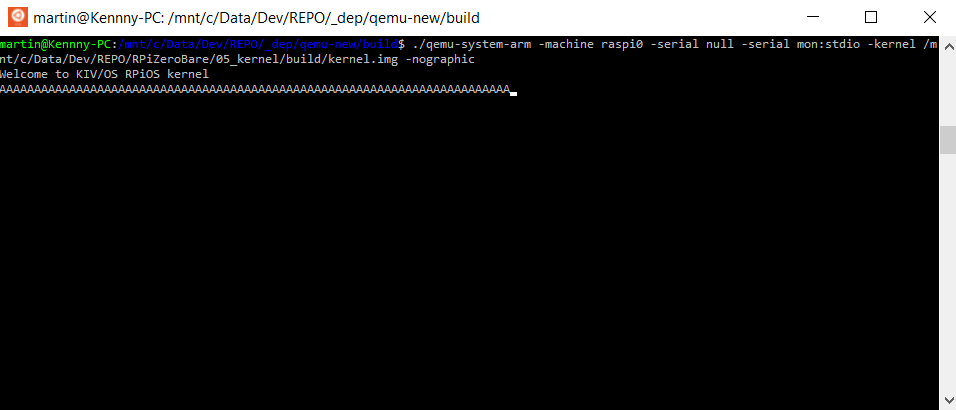
\includegraphics[width=\linewidth]{qemutest.png}
\end{figure}

Po stisknutí ctrl-A a C se přepne ovládání do konzole qemu, výstupy však pokračují dál. Pro ukončení napišme příkaz {\tt quit}, který se nejspíš bude prolínat se zapisovanými znaky {\tt A}, a potvrďme enterem.


\section{Ladění}

Pro ladění emulovaného kódu lze využít ladicí nástroj {\tt gdb}. Pro debuggování jiné, než aktuální platformy je však nutné instalovat balíkovou verzi {\tt gdb-multiarch}. Ta je dostupná ze standardních zdrojů vaší distribuce.

Emulátor qemu podporuje připojení debuggeru gdb. Je ale nutné dodat další parametry.

\begin{verbatim}
./qemu-system-arm -machine raspi0 -serial null -serial mon:stdio \
       -kernel /home/dev/kernel.img -nographic -S -gdb tcp::1234
\end{verbatim}

Nově přibyly dva parametry:
\begin{itemize}
	\item {\tt -S} -- po spuštění je emulace zastavena na první instrukci hostovaného systému, která by se provedla a bude čekat na spuštění z gdb
	\item {\tt -gdb tcp::1234} -- exportuje rozhraní pro gdb na TCP port {\tt 1234}
\end{itemize}

Volitelně lze vynechat přepínač {\tt -S}, pak se systém spustí a dovolí pouze připojení gdb do již běžícího systému.

Do emulace se pak lze připojit následujícím příkazem:
\begin{verbatim}
gdb-multiarch -ex 'set architecture arm' \
              -ex 'file kernel' \
              -ex 'target remote tcp:localhost:1234' \
              -ex 'layout regs'
\end{verbatim}

Přepínač {\tt -ex} provede příkaz konzole gdb. My potřebujeme tyto příkazy:
\begin{itemize}
	\item {\tt set architecture arm} -- pro přepnutí na architekturu a instrukční sadu ARM
	\item {\tt file kernel} -- pro propojení běžícího kódu se zkompilovaným binárním souborem
	\item {\tt target remote tcp:localhost:1234} -- pro připojení se k běžící instanci qemu na TCP portu 1234
	\item {\tt layout regs} -- volitelné -- přepnutí do pohledu, ve kterém vidíme registry a aktuální kód
\end{itemize}

Jakmile se nám povede připojit, můžeme ovládat emulaci (a debugging) např. následujícími příkazy (základní sada):

\begin{itemize}
	\item {\tt continue} (nebo jen {\tt c}) -- pokračuje v provádění příkazů, popř. spustí emulaci, pokud jsme ji vytvořili s přepínačem {\tt -S}
	\item {\tt si} -- krok o jednu instrukci
	\item {\tt s} -- krokuje tak dlouho, dokud neopustí aktuální funkci
	\item {\tt print <spec>} (nebo jen {\tt p <spec>}) -- vypíše obsah paměti na dané adrese; {\tt <spec>} může být:
		\begin{itemize}
			\item identifikátor (např. {\tt moje\_promenna})
			\item adresa prefixovaná hvězdičkou (např. {\tt *0x8000})
			\item a jiné
		\end{itemize}
	\item {\tt print/x <spec>} (nebo jen {\tt p/x <spec>}) -- totéž, ale pro výpis v hexadecimální podobě
	\item {\tt break <spec>} -- nastaví (instrukční) breakpoint na dané místo; {\tt <spec>} může být opět identifikátor, adresa prefixovaná hvězdičkou, apod.
	\item {\tt clear} -- vymaže všechny breakpointy
	\item {\tt clear <spec>} -- vymaže zadaný breakpoint
	\item {\tt quit} -- odpojí se od laděné instance qemu
\end{itemize}

Seznam příkazů pochopitelně není úplný, kompletní dokumentaci lze nalézt zde: \url{https://ftp.gnu.org/old-gnu/Manuals/gdb/html_node/gdb_toc.html}


\section{Známé problémy}

Emulace pomocí qemu není zdaleka dokonalá. Určité věci chybí, nebo jednoduše nefungují jak mají:

\begin{itemize}
	\item SYSTIMER -- systémový časovač; efektivně zamezuje použití preemptivního multitaskingu pomocí tohoto druhu časovače
	\item bezdrátový adaptér -- momentálně neexistuje oficiální cesta, jak virtualizovat/emulovat WiFi (pro variantu RaspberryPi Zero W)
\end{itemize}

\end{document}























